
\newpage
\section{Mathematical Background}%
\label{sec:background_}

\subsection{Hilbert Spaces}%
\label{ssub:hilbert_spaces}

We will in this report assume $\Omega $ to be a compact and open set in $\mathbb{R} ^{d}$.

\begin{definition}
Let $p \in \mathbb{R} $, $ 1 \le  p \le  \infty$. We define the space $L^{p}\left( \Omega  \right) $ to be the set of all measurable functions $f: \Omega  \mapsto \mathbb{R} $ such that
$\left\lvert f \right\rvert ^{p}$ is Lebesgue measurable, i.e,

\begin{equation*}
    L^{p}\left( \Omega  \right) = \left\{ f: \Omega \mapsto \mathbb{R}  \mid \int_{\Omega }^{} \left\lvert f \right\rvert ^{p} d \Omega  < \infty  \right\}
.\end{equation*}
The set of locally integrable functions for any compact subset $K \subseteq \text{Interior}\left( \Omega  \right) $ is defined as

\begin{equation*}
    L_{loc}^{1}\left( \Omega  \right)  = \left\{ f: f \in L^{1}\left( \Omega  \right)  \quad \forall K   \right\}.
\end{equation*}
\end{definition}


Let $u \in L^{p}\left( \Omega  \right) $. We define the integral norm of order $p$ to be \[
\| u \|_{ L^{p}\left( \Omega  \right)  }^{  }  = \left( \int_{\Omega }^{} \left\lvert u \right\rvert ^{p} dx  \right) ^{\frac{1}{p}}.
\]
Since $p=2$ is frequently used in this report, we also define for convenience a compact notation $\| u \|_{ \Omega  }^{  }  = \| u \|_{ L^{2}\left( \Omega  \right)  }^{  } $ .  We say that $L^{2}\left( \Omega  \right) $ is a Hilbert space if it is equipped with a inner
product of two functions $u,v \in L^{2}\left( \Omega  \right) $ such that
\[
\left( u,v \right) _{\Omega } = \left( u,v \right) _{L^2\left( \Omega  \right) } = \int_{\Omega }^{} u  v dx.
\]


We will now establish a notion of the weak derivative, but first are we going to characterize some useful definitions of continuity. The space $C^{k}\left( \Omega  \right) $ for $k\ge 0$ denotes the set of functions whose derivatives, up to order of
$k$ , is continuous in $\Omega $. Note that we often use the shorthand notation $ C^{0} = C\left( \Omega  \right)  = C^{0}\left( \Omega  \right) $.
From this, let $C^{\infty}\left( \Omega  \right) $ be the set of infinitely differentiable functions in $\Omega $. Furthermore, we then denote the space $C^{\infty}_{0}\left( \Omega  \right)$ as the space of all functions, $u \in C^{\infty}\left( \Omega
\right) $, vanishing outside of any compact subset of $\Omega $. Let $u,v \in  C^{1}\left( \Omega  \right) $ and the define boundary $\Gamma  = \partial \Omega $ with a corresponding outer normal vector $n$. It is well known that this partial
integration formula holds \cite{manzoni2021optimal},

\[
\int_{\Omega }^{} \nabla u \cdot v dx = \int_{\Gamma }^{} u\cdot v n ds - \int_{\Omega }^{} u \cdot \nabla v dx.
\]
We now use this notation for derivatives
\footnote{In literature is often $D^{\alpha } f$ commonly used, but later in the report is this notation reserved for the Hessian operator. Therefore, we then the notation $\partial ^{\alpha } f$ in this report.} so
\begin{equation}
\label{eq:mixed_derivative}
\partial ^{\alpha  } f = \frac{\partial ^{\left\lvert \alpha  \right\rvert } f}{ \partial ^{\alpha _{1} } x_{1} \partial ^{\alpha _{2}} x_{2}  }, \quad \text{where } \alpha=\left( \alpha _{1}, \alpha _{2} \right) \text{ and } f \in C^{\left\lvert \alpha  \right\rvert }
\left( \Omega  \right)
.\end{equation}
Finally, let $u \in  L^{1}_{loc}\left( \Omega  \right) $. We call the function $w \in L_{loc}^{1}\left( \Omega  \right) $ the $\alpha $-th weak derivative of $u$  if \[
\int_{\Omega }^{} w \varphi  dx = \left( -1 \right) ^{\left\lvert \alpha  \right\rvert } \int_{\Omega }^{} u \cdot \partial ^{\alpha } \varphi dx, \quad \forall \varphi \in  C_{0}^{\infty}\left( \Omega  \right).
\]

We are now able to construct the Sobolev space,

\begin{definition}[Sobolev space]
    \label{def:sobolev_spaces}
    Let $m\ge 0$ be an integer and let $1 \le  p \le  \infty$ be a real number. Then we define the Sobolev space
\[
H^{m}\left( \Omega  \right) = \left\{ u \in L^{2}\left( \Omega  \right)  \mid  \partial ^{\alpha } u \in L^{2}\left( \Omega  \right)  \forall \alpha : \left\lvert \alpha  \right\rvert  \le m \right\}.
\]
Thus, $H^{m}( \Omega ) $ is spanned by functions with derivatives of order up to $m$ in $L^{2}( \Omega ) $.
\end{definition}

\todo[inline]{ Need to define $\| \cdot  \|_{ r, \Omega  }^{  } $   }
Equipped with the inner product is $H^{m}\left( \Omega  \right) $  denoted as a Hilbert space, that is, for $u,v \in H^{m}\left( \Omega  \right) $, \[
    \left( u,v \right) _{H^{m}\left( \Omega   \right) } = \sum_{\left\lvert \alpha  \right\rvert  \le  m}^{}  \int_{\Omega }^{} \partial ^{\alpha } u \partial ^{\alpha } v dx.
\]
Similarly, the norm is is denoted as, \[
\| u \|_{ H^{m}\left( \Omega  \right)  }^{  }  = \left( \| u \|_{ L^{2}\left( \Omega  \right)    } + \sum_{k = 1}^{m}  \left\lvert u \right\rvert ^{2} _{  H^{k}\left( \Omega  \right) }\right) ^{\frac{1}{2}},
\]
where the seminorm is defined such that, \[
\left\lvert u \right\rvert _{H^{k}\left( \Omega  \right) } = \left( \sum_{\left\lvert \alpha  \right\rvert  = k}^{} \| \partial ^{\alpha }u \|_{ \Omega  }^{ 2 }  \right).
\]
For convenience, we also entitle the notation,
\[
H^{m}_{0} \left( \Omega  \right) = \left\{ \text{completion of }C_{0}^{\infty}\left( \Omega  \right) \text{ w.r.t. } \| \cdot  \|_{H^{m}\left( \Omega  \right)   }^{  }  \right\}.
\]

\todo[inline]{ Write definitions considering $H^{\frac{1}{2}}( \Gamma ) $  }



\subsection{Computational Domains}%
\label{sub:computational_domain}
Assume that $\Omega \subset \mathbb{R} ^{d} $ is a compact set.
A key element in finite element methods is to be able to discretize the domain $\Omega $ properly. Even though there exists methods handling complex geometries will we still restrict ourself some key assumptions.

First of all, if $\Omega $ has a smooth boundary, then it can be very difficult to fully discretize unless we are introducing nonlinear functions on the boundary, thus, in standard methods a key assumption is that the set $\Omega $ is a polyhedra \cite[Assumption
1.7]{pietro2012}. This is useful since a polyhedra can be fully covered by a collection of polyhedra and, hence, motivating us to define a fitted mesh .

\begin{definition}[Mesh]
   Assume that some $\Omega \subset \mathbb{R} ^{d} $ is a polyhedra.
    We define a (general) mesh $\mathcal{T} $ of the domain $\Omega $ to be a collection of disjoint polyhedra $\left\{ T \right\}  $ forming a partition of $\Omega $ s.t.\[
    \overline{\Omega } = \bigcup _{T \in \mathcal{T} } T
    \]
    We say that each $T \in  \mathcal{T} $ is a mesh element or an element.
\end{definition}

\begin{definition}[Fitted mesh]
   Assume that the set $\Omega \subset \mathbb{R} ^{d} $ is our physical domain.
   We say that the mesh is fitted if $\Omega $ can be fully covered using a general mesh.
\end{definition}

\begin{definition}[Mesh size]
We define the mesh size to is the maximum diameter $h $ of any polyhedra in the mesh $\mathcal{T} = \left\{ T \right\}  $, that is,

\begin{equation}
\begin{split}
    h _{T} & = diam\left( T \right)   = \max_{x_1, x_{2} \in T} dist(x_{1}, x_{2}),  \\
    h_{max} &= \max_{T \in \mathcal{T} }  h_{T} := h,
\end{split}
.\end{equation}
We denote $\mathcal{T} _{h}$ to be a mesh $\mathcal{T} $ with size $h$.
\end{definition}

\begin{definition}[Conform mesh]
Let $\mathcal{T}_{h} $ be a mesh of $\Omega $. We say a mesh is conform if $T_{1} \neq T_{2 }$  then $T_{1} \cap T_{2} \neq \emptyset  $ for all $T_{1}, T_{2} \in \mathcal{T}_{h}$. This means that each $T$ share either a vertex or a facet.
\end{definition}

\begin{definition}[Shape regular and quasi-uniform]
Let $\mathcal{T}_{h} $ be a mesh of $\Omega $ .
Let the chunkiness parameter $c_{T} := h_{T}/r_{T}$, where $r_{T}$  is the largest ball that be inscribed inside a element $T \in \mathcal{T}_{h} $.
We say that a mesh is shape regular if $c_{T}\le  c$ is independent of $T$  and $h$. We also say that the mesh is quasi-uniform only if it is shape regular and $h_{max} \le  c h_{min}$.
\end{definition}

\begin{assumption}
Assume that any mesh $\mathcal{T}_{h} $ is conform, shape regular and quasi-uniform.
\end{assumption}





We will generally assume that a mesh $\mathcal{T}_{h} $ is conform, shape regular and quasi-uniform unless specified.
 The fact that the mesh is conform makes is a useful property since the interface between mesh elements has come into contact in the sense
that it is either a vertex or a facet. This with the combination of shape regularity and quasi-uniformity has been a major key to prove important inequalities in broken Sobolev spaces \cite[Chapter 1.4.1]{pietro2012}. Hence, the assumptions are
very handy when proving convergence.

Questions arise when we want to allow for complex geometries where some physical domain $\Omega $ has a smooth boundary $\Gamma $ and, thus, cannot be fully covered of a fitted mesh. This motivates us to define a so-called unfitted mesh. In this
report is  to solve the problems on a unfitted mesh.

\begin{definition}[ Unfitted mesh]
 Let a background domain $\widetilde{\Omega } \subset \mathbb{R} ^{d} $ have a corresponding mesh $\widetilde{\mathcal{T} _{h}}$.
Assume that the set $\Omega\subset   \widetilde{\Omega }  $ is a physical domain with a corresponding smooth boundary $\Gamma$. We define the unfitted mesh as the mesh that intersects the interior of $\Omega$, i.e., the intersection $\widetilde{\mathcal{T}_{h} } \cap
 \Omega^{\circ }     $ where $ \Omega ^{\circ } = \Omega \setminus \Gamma  $.
\end{definition}

\todo[inline]{ Maybe illustrate using figures. Check \cite[Fig 2.5]{pietro2012}  }

\begin{definition}[Facets]
Let $\mathcal{T}_{h}  = \left\{ T \right\} $ be a mesh of $\Omega \subset  \mathbb{R} ^d $ consisting of polygons $T \in \mathbb{R} ^{d}$.
The set of all facets is the union of external and internal facets, $\mathcal{F} _{h} = \mathcal{F} ^{ext}_{h} \cup \mathcal{F} _{h}^{int} $, where each are defined like this:
\begin{enumerate}[label=\arabic*)]
    \item We denote the set of interior facets as \[
            \mathcal{F}^{int} _{h} = \left\{ F=T^{+}\cap T^{-}  \mid  T^{+}, T^{-} \in \mathcal{T}_{h}  \right\}
\]
\item We denote the set of exterior facets as
\[
            \mathcal{F}^{ext} _{h} = \left\{ F= \partial T \cap \partial \Omega    \mid  T  \in \mathcal{T}_{h}  \right\}
\]
\end{enumerate}
\end{definition}


\begin{definition}[Normal vector ]
Let $\mathcal{T}_{h} $ be a mesh of $\Omega $ equipped with the facets $\mathcal{F}_{h} $. We will define the following normal vectors
\begin{enumerate}[label=\arabic*)]
    \item We define $n \mid _{T}$ to be unit outward normal on $\partial T$ for each $T \in \mathcal{T}_{h} $
 \item For all $F \in \mathcal{F }^{int} _{h}$ we define $n$ to be the facet normal $ n  \mid_F = n \mid _{T^{+}} $  from $T^{+}$ to $T^{-}$, illustrated in figure \ref{fig:normal}.
 \item For all $F \in F^{ext}_{h}$ we define the facet normal $n \mid _{F} = n \mid _{T} $ to the unit outward normal.
\end{enumerate}
Keep in mind that in many that we often will simply use the notation $n = n \mid _{T}$ in most cases.
\end{definition}

\begin{definition}[Jump and average]
    Let $v\in L^2( \Omega ) $ be a scalar function on $\Omega$ with a corresponding shape regular and quasi-uniform mesh $\mathcal{T}_{h} $. We will use the following definitions
    \begin{enumerate}[label=\arabic*)]
        \item Let $F \in \mathcal{F}^{int} _{h}$ and $v^{\pm}| _{F} = \lim_{t\to 0} v( x \pm tn)   $ for $x \in F$. We define the mean as $\mean{ v} |_{F} = \frac{1}{2} (v^{+}_{F} + v^{-}_{F})   $ and the jump as $\jump{v}|_{F} =  v^{+}_{F} - v^{-}_{F} $.
        \item Let $F \in \mathcal{F}^{ext} _{h}$ and let $ v( x) =  v(x)|_{F} $ for  $x \in F$.
We define the mean as $\mean{ v} |_{F} = v    $ and the jump as $\jump{v}|_{F} = v$.

    \end{enumerate}
    To simplify will we use the notation $\mean{ v } = \mean{ v } \mid _{F}    $ and $\jump{ v } = \jump{ v } \mid _{F}    $ for all $F \in \mathcal{F} _{h}$.

\end{definition}




\begin{figure}[!h]
\centering
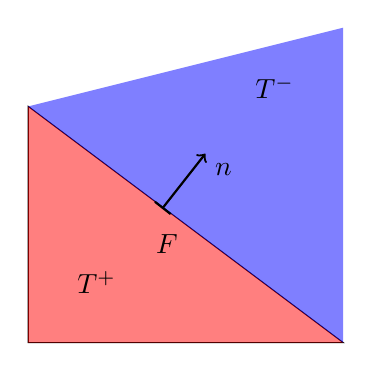
\begin{tikzpicture}[scale=1]
\coordinate (A) at (0,0);
\coordinate (C) at (0,3);
\coordinate (B) at (4,0);
\coordinate (D) at (4,4);
\coordinate (Tm) at (3.5,3.5);
\coordinate (Tp) at (0.5, 0.5);
\coordinate (e) at (1.5, 1.5);
\coordinate (start) at (1.7, 1.7);
\coordinate (end) at (2.25, 2.4);

\draw (A) -- (B) -- (C) -- cycle;
\fill[red, opacity=0.5] (A) -- (B) -- (C);
\fill[blue, opacity=0.5] (B) -- (C) -- (D);
\node[below left] at (Tm) {$T^{-} $ };
\node[above right] at (Tp) {$T^{+}$ };
\node[below right] at (e) {$F$ };

\draw [|->, thick] (start) -- (end);
% \node[above right] at (A) {A };
% \node[below right] at (B) {B};
% \node[above right] at (C) {C };
% \node[below right] at (D) {D};
\node[below right] at (end) {$n$};
\end{tikzpicture}

\caption{Facet $F \in \mathcal{F}_h $ shared by the triangles $T^{+}, T^{-} \in \mathcal{T}_{h} $ and the normal unit vector $n$.  }
    \label{fig:normal}
\end{figure}

\begin{lemma}[Magic formula]
    \label{lemma:magic_formula}
    Let $u,v \in L^2( \mathcal{T}_{h} ) $ then this hold,
    $  \jump{ uv }    = \jump{ u }   \mean{ v }    + \mean{ u }  \jump{ v }     $.
\end{lemma}
\begin{proof}
    The proof is quite straight forward.
    \[
        \begin{split}
    \jump{ uv }   & = u^{+}v^{+} - u^{-}v^{-} \\
     & =  \frac{1}{2}(v^{+} + v^{-})( u^{+} - u^{-})+ \frac{1}{2}(u^{+} + u^{-})( v^{+} - v^{-})   \\
     & =  \jump{ u }   \mean{ v }    + \mean{ u }  \jump{ v }
        \end{split}
    \]
\end{proof}


\subsection{Broken Sobolev spaces}%
\label{sub:broken_sobolev_spaces}

In this work will we compute norms on discontinuous elements, thus, it will be necessary to define broken Sobolev spaces. What we know is that if $T$ is a polyhedra, then the definition of $H^{m}( T)$ is covered by definition
\ref{def:sobolev_spaces}. We will now precisely define it for a collection of polyhedra $\mathcal{T}_{h}$.

\begin{definition}[Broken Sobolev spaces]
Let $\mathcal{T}_{h} $ be a mesh of some domain $\Omega  $ and some integer $m\le n$. Then we define the broken Sobolev space to be \[
H^{m}( \mathcal{T}_{h} ) := \left\{ v \in L^2( \Omega )  \mid \ v|_{T} \in H^{m}( T) \quad     \forall T \in  \mathcal{T} \right\}
\]
and similarly for the facets $\mathcal{F}_{h} $, that is
\[
    \begin{split}
        L^{2}( \mathcal{F}_{h} ) &:= \left\{ v \in L^2( \mathcal{T}_{h}  )  \mid   \ v|_{F} \in L^{2}( F)  \quad  \forall F \in  \mathcal{F}_{h}   \right\} \\
        H^{m}( \mathcal{F}_{h} ) &:= \left\{ v \in L^2( \mathcal{F}_{h}  )  \mid   \ v|_{F} \in H^{m}( F)  \quad  \forall F \in  \mathcal{F}_{h}   \right\}
    \end{split}
\]
\todo[inline]{ I am not happy with $L^2( \mathcal{F} _{h}) $ definition. }
\end{definition}
This motivates us to define broken Sobolev norms and inner products using a summation over mesh elements. That is,
\[
 \| v \|_{H^{m}( \mathcal{T} ) }^{2} = \sum_{T \in  \mathcal{T}_{h} }^{} \| v  \|_{ H^{m}( T ) }^{2  } \quad \text{ and } \quad
 (v ,w )_{H^{m}( \mathcal{T} ) }^{} = \sum_{T \in \mathcal{T} _{h}}^{} (v ,w )_{ H^{m}( T ) }^{  } .
\]
We often use the more compact notation in $L^{2}$  $\| v \|_{\mathcal{T}_{h}} =  \| v \|_{L^{2}( \mathcal{T}_{h} ) }$ and  $(v ,w )_{ \mathcal{T} }^{} = (v ,w )_{L^2( \mathcal{T} ) }^{} $.

That is,
\[
 \| v \|_{H^{m}( \mathcal{F}_{h} ) }^{2} = \sum_{F \in  \mathcal{F}_{h} }^{} \| v  \|_{ H^{m}( F ) }^{2  } \quad \text{ and } \quad
 (v ,w )_{H^{m}( \mathcal{F} ) }^{} = \sum_{T \in \mathcal{F} _{h}}^{} (v ,w )_{ H^{m}( F ) }^{  } .
\]
And again, we often use the more compact notation $\| v \|_{\mathcal{F}_{h}} =  \| v \|_{L^{2}( \mathcal{F}_{h} ) }$ and  $(v ,w )_{ \mathcal{F} }^{} = (v ,w )_{L^2( \mathcal{F}_{h} ) }^{} $.


A very useful lemma when working on estimates on broken Sobolev spaces is that a if a function is continuous, then the jump between the mesh elements is zero.
\begin{lemma}
    A function $ v \in  H^{1}( \mathcal{T}_{h} ) $ belongs to $ H^{1}( \Omega )  $ if and only if \[
    \jump{ v }   = 0, \quad F \in \mathcal{F}^{int}_{h}
    \]
\end{lemma}
\begin{proof}
    See \cite[Lemma 1.23]{pietro2012}.
\end{proof}



\subsection{Useful inverse estimates}%
\label{sub:useful_inverse_estimates}


\begin{lemma}[Local inverse estimate]
    \label{lemma:local_inverse_estimates}
    Let $v \in \mathcal{P}^{k} ( T)  $ for an element in $\mathcal{T}_{h} $ and let $F \in \mathcal{F}_{T} := \left\{ F_{h} \in \mathcal{F} _{h} : F \cap \partial T \right\}  $. Then is \[
    \| \partial _{n} v \|_{ F   }^{  } \le  C_{I} h_{T}^{-\frac{1}{2}} \| \nabla v \|_{  T}^{  }
    \]
    Here does the constant $C_{I}>0$ depend on the dimension $d$, shape regularity of $\mathcal{T}_{h} $ and the degree $k$.
\end{lemma}

\begin{proof}
    TODO: Find proof
\end{proof}

\begin{lemma}[Cauchy-Schwarz inequality]
    \label{lemma:cauchy-schwarz}
    \[
     \| ab \|_{  }^{  }  \le \| a \|_{  }^{  } \| b \|_{  }^{  }
    \]
\end{lemma}
\begin{proof}
    TODO: find proof
\end{proof}

\begin{lemma}[Second order global inverse inequality]
    \[
     \frac{1}{h}\| \partial _{nn}  v_{h} \|_{\mathcal{F}_{h}   }^{2  }  \le C_{j} \| D ^2 v_{h} \|_{ \mathcal{T} _{h} }^{ 2 }   \\
    \]

\end{lemma}
\begin{proof}
    TODO: find proof
\end{proof}
\begin{lemma}[Youngs $\varepsilon $-inequality ]
    \label{lemma:youngs_epsilon}
   \[
     2ab \le \varepsilon a^2+ b^2 \frac{1}{\varepsilon }
   \]
\end{lemma}
\begin{proof}
    TODO: find proof
\end{proof}



\subsection{Lax-Milgram lemma}%
\label{sub:lax_milgram_lemma}


\begin{definition}[Linear bounded functional]
    \label{def:linear_function}
Let $X$ be a Hilbert space. Furthermore, we define the dual space the be the space of linear and bounded functionals $F: X  \mapsto \mathbb{R} $, i.e., \[
X'  =
\left.
\begin{cases}
F: X  \mapsto \mathbb{R} \text{ s.t. }\forall v,w \in X, \forall a,b \in \mathbb{R} \text{ and } C> 0 \text{ is }   \\
  F\left( \lambda v + \mu w  \right) = \lambda F(v) + \mu F(w) \text{ and } \left\lvert F\left( v \right)  \right\rvert \le C \| v \|_{ X  }^{  }
\end{cases}
  \right\}
\]
% and we equip it with the functional norm,  \[
%     \| F \|_{ \mathcal{V} ^{*} }^{  } = \sup_{v \in \mathcal{V}   } \frac{\left\lvert F\left( v \right)  \right\rvert }{\| v \|_{ \mathcal{V}  }^{  } }.
% \]
\todo[inline]{ Maybe write it in terms of $\mathcal{L} $ definition instead. Might need to do some dive into functional analysis books. Anyhow, I am not happy with this definitionin context with the rest of the subchapter.}
\end{definition}

\begin{definition}[Bilinear bounded functional]
    \label{def:bilinear_function}
    Write definitions of a bilinear bounded operator
\end{definition}

\begin{problem}[Abstract linear problem]
    \label{def:abstract_linear_problem}
    Assume $X$ and $Y$  to be two Hilbert spaces. Let the vector space $\mathcal{L}( X,Y)  $ be all linear bounded operators spanned from $X$ to $Y$. We define the abstract linear problem as follows; find $u \in X$ s.t. \[
    a( u,v)  = l(v ) := \left<f,v \right>_{X' , X}  \forall v \in X
    \]
    Where $a \in  \mathcal{L} ( X \times X,\mathbb{R} ) $ is a bounded linear form and $f \in X':= \mathcal{L} ( X,\mathbb{R} )  $ is a bounded linear form. Here we denote $\left<\cdot ,\cdot  \right>_{X' .X} $ as the duality pairing between $X' $
    and $X $.

\end{problem}


\begin{definition}[Coercivity]
    \label{def:coercivity}
    Let $X$ be a Hilbert space and let $a \in  \mathcal{L} ( X \times  X,\mathbb{R} )  $. We say that the bilinear form $a$ is coercive on $X$ if there exists an constant $C > 0 $ s.t. \[
     a( v,v) \ge  C \| v \|_{ X }^{  } \quad  \forall v \in  X
    \]
\end{definition}


\begin{lemma}[Lax-Milgram]
    \label{def:lax-milgram}
    We say that the abstract linear problem \ref{def:abstract_linear_problem} is well-posed if $a$ is coercive. Moreover, the following a priori estimate holds true.\[
    \| v \|_{ X }^{  } \le \frac{1}{C} \| f \|_{ X'  }^{  }
    \]
\end{lemma}
\begin{proof}
    The problem can easily be proved using a special case of the Banach–Nečas–Babuška theorem. See \cite[Lemma 1.4]{pietro2012}
\end{proof}



\subsection{Finite element method}%
\label{sub:finite_element_method}


The finite element method (FEM) is a numerical method to solve partial differential equation by finding an approximation of the Problem \ref{def:abstract_linear_problem}.  Let $X_{h}$ be a finite-dimensional (polynomial) approximation space on the mesh
$\mathcal{T} _{h}$. We say that a method is conform if $X_{h}\subset X $ and non-conform if $X _{h} \not\subset X$. We define the approximate problem as follows.
\begin{problem}[The approximate problem]
    \label{def:approx_problem}
    Find  $u \in X_{h}$ s.t. \[
    a_{h}(u,v ) = \left<f,v \right>   \forall v \in X_{h}
    \]
\end{problem}

We denote the functional $a_{h}: X_{h} \times X_{h} \to \mathbb{R} $ as an consistent approximation of $a: X \times X \to \mathbb{R} $, and similarly for the right-hand side.


\begin{definition}[Broken polynomial spaces]
    Let $\mathcal{T}_{h} $ be a mesh of $\Omega \in \mathbb{R} ^{d} $. Let $\mathcal{P}^{k}(T) $ be the space of all polynomials of degree $k$ in the mesh element $T$. We define the broken polynomial space as \[
    \mathcal{P}^{k} ( \mathcal{T}_{h} ) := \left\{ v \in L^2( \Omega )  \mid  v|_{T} \in \mathcal{P}^k( T) \quad  \forall T \in  \mathcal{T}_{h}   \right\}.
    \]
\end{definition}


Assume that $V_{h} = \mathcal{P} ^{k}( \mathcal{T} _{h}) $ is spanned by the polynomial basis $\left\{ \phi _{1}, \ldots, \phi _{N}  \right\} $ s.t. $dim(V_{h}) = N$. We can then define $u = \sum_{i=1}^{N}  U_{i} \phi_{i} $ with coefficients $\left\{
U_{i}\right\} _{i=1}^{N}$ and the stiffness matrix $\left[ \mathcal{A}  \right] _{ji} = a_{h}( \phi _{i}, \phi _{j}) $ and vector $\left[ f \right] _{j} = l_{h}( \phi_{j} ) $. Thus we have the following equivalent discrete system of the Problem
\ref{def:approx_problem}. The goal is to find $U \in \mathbb{R} ^{N}$ s.t.  \[
\mathcal{A} U =F.
\]
\todo[inline]{ Write something about coercivity and boundedness. }

We may recall the basic the discrete $l^{p}$ norm, i.e.,\[
    \| U  \|_{ p }^{  } = \sum_{i=1}^{N}  \abs{ U_{i}  } \text{ for } U \in \mathbb{R} ^{N}
,
\]
where $1\le p < \infty$ and $\| U \|_{ \infty }^{  }  = \max_{i}  \abs{ U_i } $.
To not confuse with Sobolev spaces will we generally denote the notation $\| \cdot  \|_{ \mathbb{R} ^{N} }^{  } := \| \cdot  \|_{ 2 }^{  }   $ for the discrete $l^2$-norm.
From basic theory is the matrix norm defined as \[
\| \mathcal{A}  \|_{ \mathbb{R} ^{N} }^{  }  = \max_{U \in \mathbb{R} ^{N} \setminus 0} \frac{\| AU \|_{ \mathbb{R} ^{N} }^{  } }{\| U \|_{\mathbb{R} ^{N}  }^{  } } \text{ for } \mathcal{A} \in \mathbb{R} ^{N\times N}.
\]
Assume that $\mathcal{A} $ is invertible, then we define the condition number s.t., \[
\kappa ( \mathcal{A} ) = \| \mathcal{A}  \|_{ \mathbb{R} ^{N} }^{  } \| \mathcal{A} ^{-1} \|_{ \mathbb{R} ^{N} }  .
\]







